\documentclass[border=0.8ex,svgnames,tikz]{standalone}
\usepackage{amsmath,mathtools}
\usepackage{fontspec}
\setmainfont{Source Serif 4}
\setsansfont{Source Sans 3}
\setmonofont{Source Code Pro}
\begin{document}
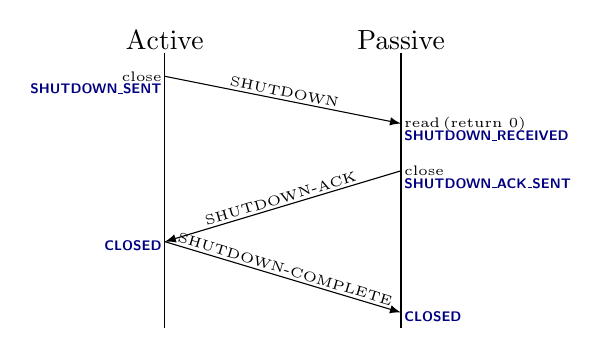
\begin{tikzpicture}[
  every label/.style={font=\tiny},
  every node/.style={inner sep=1pt,above,sloped,font=\tiny},
  status node/.append style={text=NavyBlue,font=\tiny\sf\bfseries},
  ]
  \path[draw] (0,0) coordinate(active-begin)
    node[above,font=\normalsize]{Active} -- (0,-3.5);
  \path[draw] (active-begin)
    ++(0,-0.3) coordinate[label=left:{close}](active-close)
    ++(0,-2.1) coordinate(active-shutdown-sent);
  \path (active-close)         ++(0,-0.16) node[left,status node]{SHUTDOWN\_SENT}
        (active-shutdown-sent) ++(0,-0.05) node[left,status node]{CLOSED};

  \path[draw] (3,0) coordinate(passive-begin)
    node[above,font=\normalsize]{Passive} -- (3,-3.5);
  \path[draw] (passive-begin)
    ++(0,-0.9) coordinate[label=right:{read\,(return 0)}](passive-read)
    ++(0,-0.6) coordinate[label=right:{close}](passive-close)
    ++(0,-1.8) coordinate(passive-closed);
  \path (passive-read)   ++(0,-0.16) node[right,status node]{SHUTDOWN\_RECEIVED}
        (passive-close)  ++(0,-0.16) node[right,status node]{SHUTDOWN\_ACK\_SENT}
        (passive-closed) ++(0,-0.05) node[right,status node]{CLOSED};

  \path[draw]
    (active-close)         edge[-latex] node{SHUTDOWN}     (passive-read)
    (passive-close)        edge[-latex] node{SHUTDOWN-ACK} (active-shutdown-sent)
    (active-shutdown-sent) edge[-latex] node{SHUTDOWN-COMPLETE} (passive-closed);
\end{tikzpicture}
\end{document}
